% write your paper in here

\chapter{Genome assembly of the coral \textit{Astrangia poculata}}

\section{Introduction}

The species \textit{Astrangia poculata} \cite{peters1988nomenclature}, also called the Northern star coral, is a temperate hard coral distributed across a wide range of latitudes in the western Atlantic ocean \cite{dimond2013simple}. It belongs to the class Anthozoa, a division of cnidarians that includes hard corals, soft corals, and sea anemones. Along with its adaptation to temperature variations, this coral has a facultative symbiosis with algae from the family Symbiodiniaceae, making it a compelling model to study coral response to environmental changes. To this end, we assembled its genome which will constitute a resource for downstream analysis. The genome had previously been assembled with a combination of Illumina and Hi-C reads; although this first version was highly contiguous, its size was excessively small compared to the expected genome size, and the draft had a poor completeness. I assembled the genome \textit{de novo} with newly sequenced Nanopore reads, which I combined with Illumina and Hi-C reads to produce an improved reference sequence. 

\section{Material \& Method}

\subsection{Sequencing data}

High-molecular-weight DNA was extracted by Dovetails Genomics. The sample was further purified with AMPure XP beads and fragments were selected on their size with Circulomics Short Reads Eliminator XS. \\
A Nanopore library was prepared with the Ligation Sequencing Kit LSK109, starting with 2.1 {\textmu}g of DNA, and yielded 1.4 {\textmu}g of DNA. The library was sequenced with a MinION on a R9.4 flowcell, with fast Guppy v4 basecalling. The flowcell was washed and reloaded three times (281 ng of DNA for the first load, 187 ng for subsequent loads) and ran for 89 hours. A total output of 6.79 Gb was obtained with an N50 of 18 kb and an N90 of 5 kb (Table \ref{tab:apoculata_datasets}). Adaptors were removed using Porechop \cite{porechop} with default parameters. After trimming, the dataset reached 6.77 Gb. \\

Dovetails Genomics produced two shotgun Illumina datasets of paired-end 150 bp reads: one with 414 million reads and an estimated insert size of 395 bp, and the second with 235 million reads and an estimated insert size of 484 bp (Table \ref{tab:apoculata_datasets}). Adaptors were removed using  cutadapt \href{https://github.com/marcelm/cutadapt}{github.com/marcelm/cutadapt}. \\

Dovetails Genomics also provided three Hi-C libraries with 198 million, 266 million and 257 million paired-end 150 bp reads (Table \ref{tab:apoculata_datasets}). The reads were trimmed of the adaptors with cutadapt.\\

\begin{table}[H]
\centering
\caption{\textit{Astrangia poculata} sequencing datasets.}
\begin{tabular}{|l|l|l|l|}
\hline
\textbf{Reads} & \textbf{Length} & \textbf{N50} & \textbf{Size} \\
\hline
Hi-C & 2*150 bp & - & 217 Gb \\
Illumina & 2*150 bp & - & 195 Gb\\
Nanopore & - & 18 kb & 7 Gb \\
\hline
\end{tabular}
\label{tab:apoculata_datasets}
\end{table}

\subsection{Genome size estimation}

Dovetails Genomics estimated the genome size to 462 Mb. I estimated the genome size using the second shotgun Illumina dataset of 235 million reads and the module kmercount.sh from BBtools \cite{bbtools}; the tool predicted a haploid size of 453 Mb, a ploidy of 2, and 40.95\% of repeats. 

\subsection{Genome assembly}

Five assemblers were tested with default parameters: Canu \cite{canu}, Ra \cite{ra}, Raven \cite{raven}, Flye \cite{flye}, wtdbg2 \cite{wtdbg2}. Purge Haplotigs \cite{purge_haplotigs} was run on the wtdbg2 assembly with default parameters, using the full shotgun Illumina datasets mapped with bowtie2 \cite{bowtie2}. The wtdbg2 assembly was polished with HyPo \cite{hypo}, using the full shotgun Illumina datasets mapped with bowtie2. Hi-C reads were mapped to the wtdbg2 assembly and processed using hicstuff \cite{hicstuff}, available at \href{https://github.com/koszullab/hicstuff}{github.com/koszullab/hicstuff}, with the parameters -{}-enzyme DpnII -{}-iterative -{}-aligner bowtie2. The draft assembly was then scaffolded using instaGRAAL \cite{instagraal}, with default parameters (-{}-levels 4 -{}-cycles 100 -{}-coverage-std 1, -{}-neighborhood 5). The output was refined with the module instaGRAAL-polish. \\

\subsection{Assembly evaluation}

BUSCO v4 \cite{busco_evaluation} was run against metazoa odb10 (954 features) without the parameter -{}-long. \textit{k}-mer completeness was calculated by running KAT comp v2.4.2 \cite{kat_evaluation} with the full shotgun Illumina datasets. The contact map was built using the hicstuff pipeline, with the three Hi-C libraries, and hicstuff view with the parameter \texttt{-{}-binning 200}. \\

\section{Results}

The assembly provided by Dovetails Genomics had chromosome-level scaffolds, but one of its major flaws was that its total size only reached 252 Mb (Table \ref{tab:apoculata_assembly_stats}) whereas the genome size was estimated to 462 Mb by Dovetails Genomics and to 453 Mb by BBtools. \\

\begin{table}[H]
\caption{Basic statistics of \textit{Astrangia poculata} assemblies, presenting the strategies that were used for each assembly (purging haplotigs, assembly polishing, scaffolding), assembly size, number of contigs, N50, number of BUSCO single complete features and BUSCO duplicate complete features.}
\resizebox{\columnwidth}{!}{
\begin{tabular}{lcccccccc}
\hline
\multirow{2}{*}{\textbf{Assembler}} & \multirow{2}{*}{\textbf{Purging}} & \multirow{2}{*}{\textbf{Polishing}} & \multirow{2}{*}{\textbf{Scaffolding}} & \multirow{2}{*}{\textbf{Assembly}} & \multirow{2}{*}{\textbf{\# contigs}} & \multirow{2}{*}{\textbf{N50}} & \multicolumn{2}{c}{\textbf{BUSCO}} \\
    &  &  &  & \textbf{size} &  &  & \textbf{single} & \textbf{dup.} \\
\hline
Dovetails & - & - & - & 252 Mb & 7848 & 16.8 Mb & 60.0\% & 0.2\% \\
\hline
Canu & $\times$ & $\times$ & $\times$ & 597 Mb & 8317 & 97 kb & 56.0\% & 7.9\% \\
\hline
Flye & $\times$ & $\times$ & $\times$ & 719 Mb & 7259 & 167 kb & 67.9\% & 8.9\% \\
\hline
Ra & $\times$ & $\times$ & $\times$ & 271 Mb & 2851 & 115 kb & 43.9\% & 0.3\% \\
\hline
Raven & $\times$ & $\times$ & $\times$ & 400 Mb & 2912 & 172 kb & 52.3\% & 0.4\% \\
\hline
wtdbg2 & $\times$ & $\times$ & $\times$ & 476 Mb & 4423 & 439 kb & 55.1\% & 0.3\% \\
    & \checkmark & $\times$ & $\times$ & 452 Mb & 2995 & 475 kb & 54.6\% & 0.3\% \\
    & \checkmark & \checkmark & $\times$ & 458 Mb & 2995 & 480 kb & 87.7\% & 2.4\% \\
    & \checkmark & \checkmark & \checkmark & 458 Mb & 488 & 31.0 Mb & 89.1\% & 1.2\% \\
\hline
\end{tabular}
}
\label{tab:apoculata_assembly_stats}
\end{table}

Ra and Raven both produced smaller assemblies than expected, with the Ra assembly size close to the one of Dovetails Genomics. Canu and Flye both produced assemblies quite larger than expected, which is likely due to uncollapsed haplotypes, as is shown by the increased percentages of duplicated BUSCO complete features. wtdbg2 produced the most convincing draft, with an assembly size close to expectations and the highest N50. Purge Haplotigs reduced the number of contigs from 4423 to 2995 and slightly increased the N50 from 439 kb to 475 kb. After polishing, the overall number of complete BUSCOs went from 54.9\% to 90.1\%. Scaffolding with instaGRAAL yielded 14 chromosome-level scaffolds, with sizes ranging from 21.1 Mb to 54.8 Mb. The final assembly contains 14 scaffolds and, after removing small sequences, has a size of 455 Mb and a BUSCO completeness of 90.4\%. The KAT plot shows two peaks, as the species is diploid \ref{fig:coral_kat}. Low multiplicity (or erroneous) \textit{k}-mers are absent from the assembly, as expected. A part of heterozygous \textit{k}-mers are represented once in the assembly and the rest are not, as only one haplotype is represented for heterozygous regions in collapsed haploid assemblies. The majority of homozygous \textit{k}-mers are represented once, although there are some missing and duplicated \textit{k}-mers. \\

\begin{figure}[H]
    \centering
    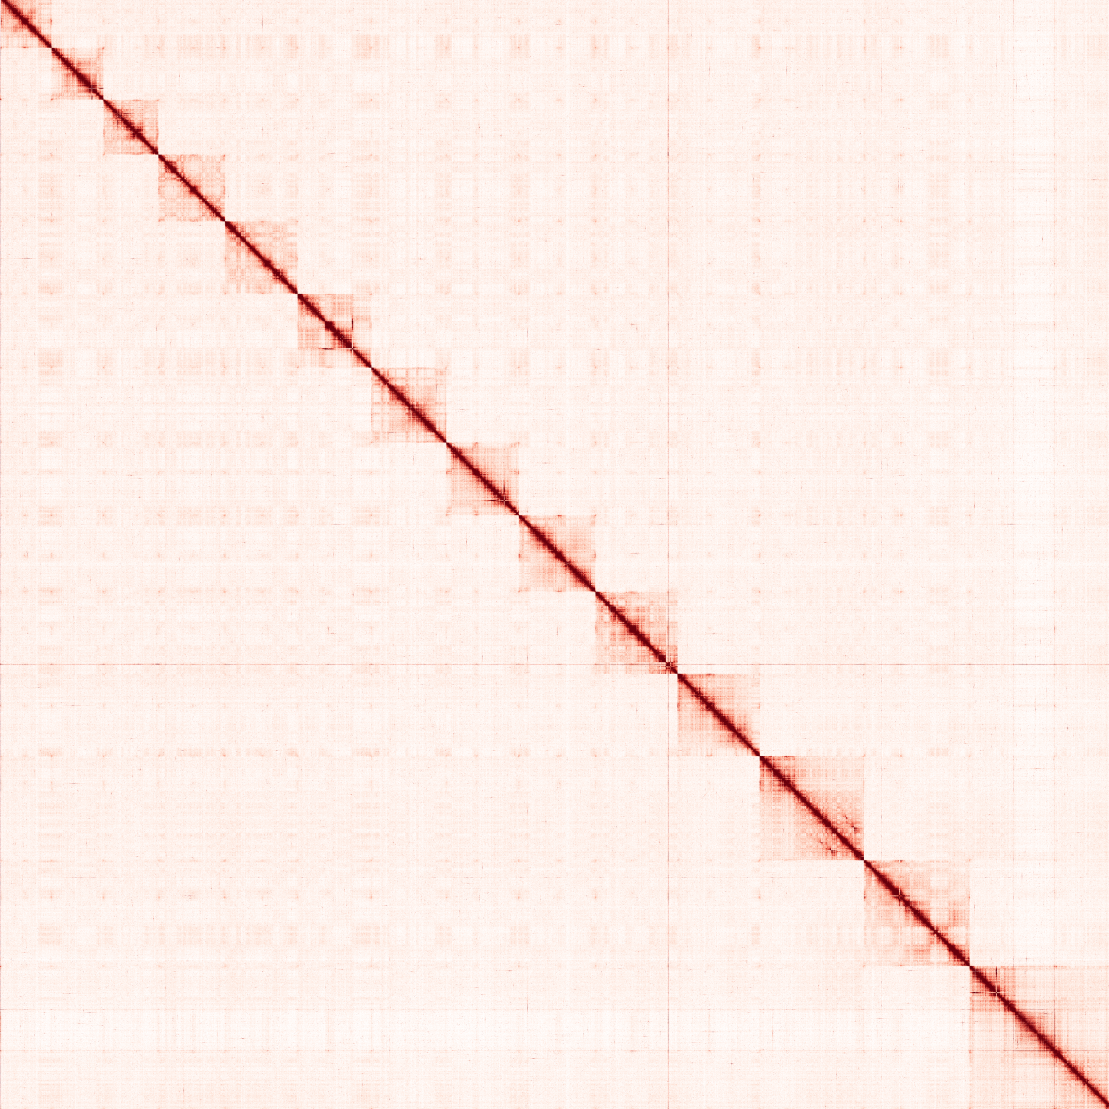
\includegraphics[width=0.9\linewidth]{fig/apoculata_contact_map_bin200.png}
    \caption{Contact map representing the 14 chromosome-level scaffolds of the final assembly (combining wtdbg2, Purge Haplotigs, HyPo and instaGRAAL).}
    \label{fig:coral_contact_map}
\end{figure}

\begin{figure}[H]
    \centering
    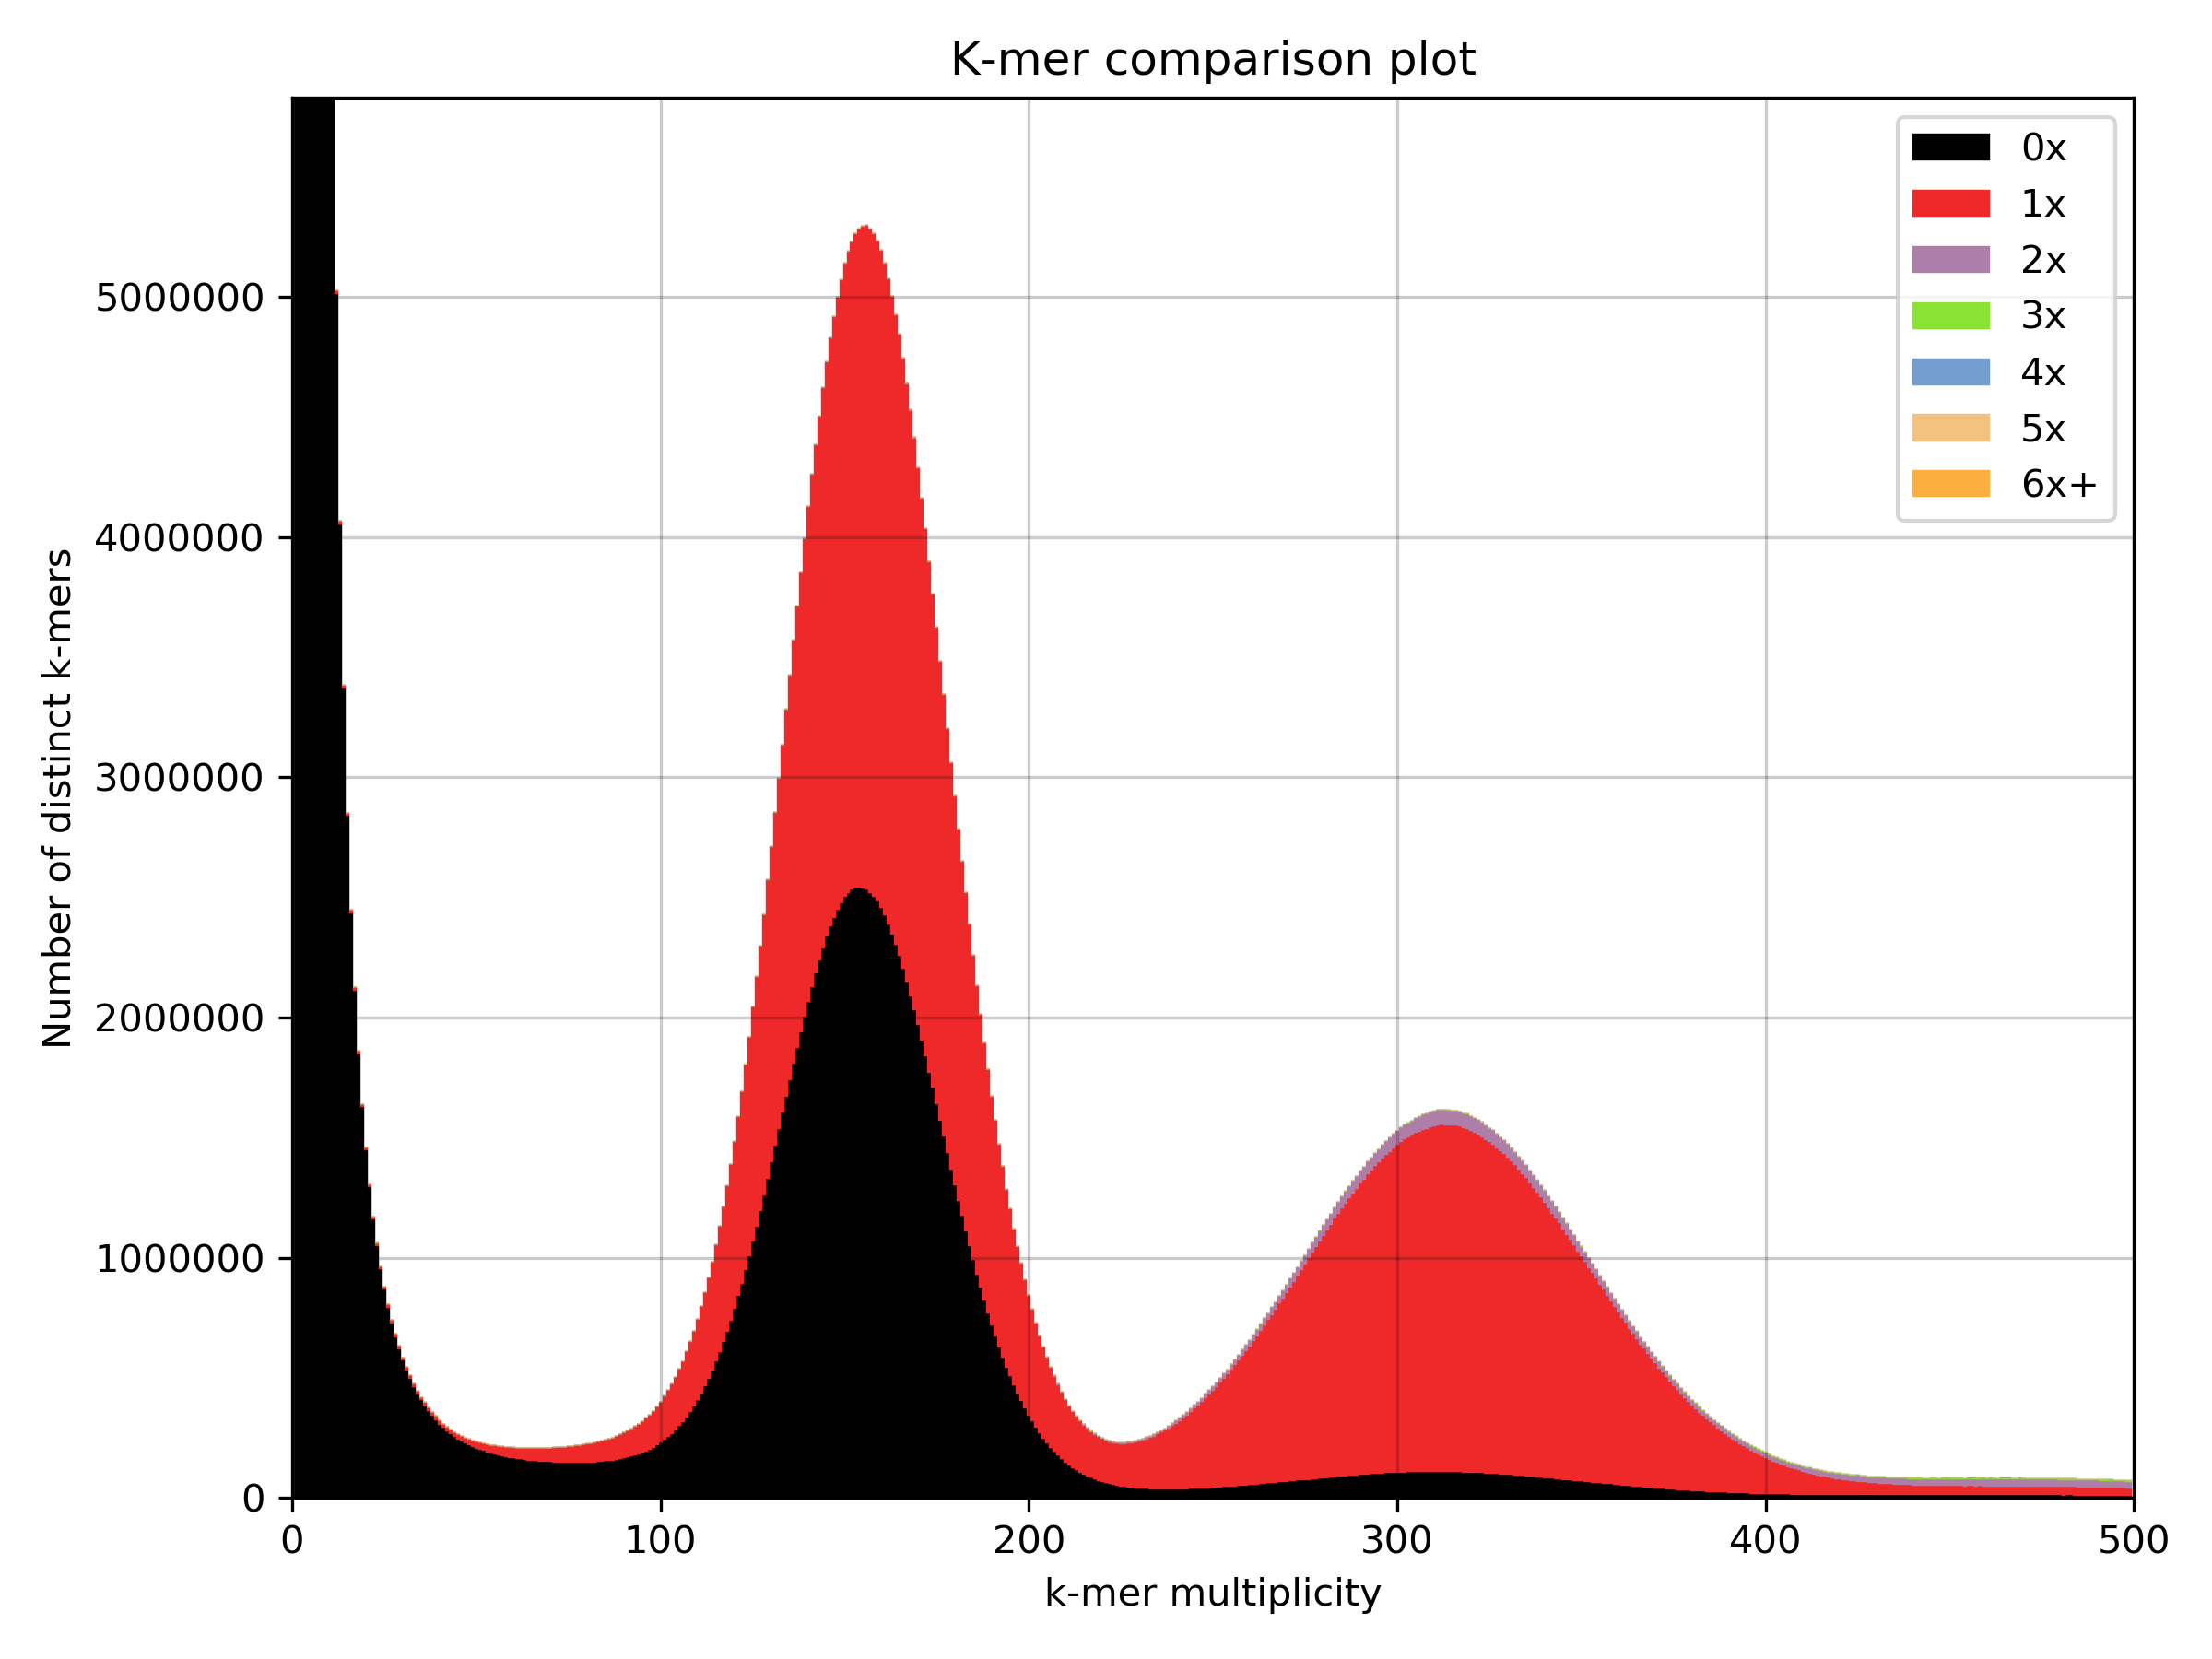
\includegraphics[width=0.9\linewidth]{fig/coral_kat.png}
    \caption{\textit{k}-mer analysis of the chromosome-level scaffolds of \textit{Astrangia poculata}. }
    \label{fig:coral_kat}
\end{figure}

\section{Discussion}

The initial assembly of \textit{Astrangia poculata} reached a high contiguity, but its small size and completeness indicated that the assembly was incomplete. The new assembly has a size and a number of chromosome-level scaffolds within the expected range, as well as high BUSCO and \textit{k}-mer completeness. This demonstrates that, although Hi-C scaffolding is a robust method to achieve chromosome-level assemblies, the quality of the input contigs is crucial. In this case, the small size of the initial assembly may result from the high repetitive content (estimated to 40.95\%) which is typically poorly handled by short reads; repeats are better resolved by long reads as their length can cover full repetitive regions \cite{pollard2018}. Interestingly, a low coverage of long reads (about 15X) was sufficient to yield an assembly with a size close to the estimated genome size, and polishing with a high-coverage short read dataset further improved the completeness. \\

Among assemblies of anthozoan genomes, only a few reached chromosome-level scaffolds: \textit{Acropora millepora}, \textit{Xenia} sp., and the assembly of \textit{Astrangia poculata} presented here (Table \ref{tab:anthozoans}). The most recent version of \textit{Acropora millepora} combines long reads, linked reads and genetic maps, while \textit{Xenia} sp. and \textit{Astrangia poculata} were both obtained with long reads, short reads, and Hi-C. One genome was scaffolded with an alternative \textit{in vitro} Hi-C protocol, called CHICAGO, but this approach led to a poor contiguity, and regular Hi-C should be favored for chromosome-level assemblies. Many genomes of hard corals (Scleractinia) were assembled with Illumina reads and scaffolded with mate pairs, and particularly for a large genomic analysis of their adaptation to elevated temperatures \cite{acropora_digitifera2}. All these assemblies have a size around 400 Mb, an overall BUSCO completeness over 88\% with few duplicated BUSCO features, and several have an N50 over 1 Mb. These assemblies, although obtained with short reads only, do not have the same flaws as the initial assembly of \textit{Astrangia poculata}, suggesting that short reads are still relevant to yield high-quality draft assemblies when combined with efficient assemblers (Platanus, in this case). Besides, the contiguity and completeness of the short-read only assemblies are comparable or higher compared to assemblies that included long reads. Hi-C scaffolding could be highly beneficial for the study of these genomes, as species of the genus Acropora have an endosymbiosis with zooxanthellae and Hi-C scaffolding can tell apart these different genomes. \\

The quality of the assembly of \textit{Astrangia poculata} makes it a new reliable reference among anthozoan genomes for downstrean analysis and comparison with other species. \\

%However, the high-molecular-weight DNA extraction and Hi-C library preparations were performed by a private company, thus no protocols are available which could have been used as a resource for other coral genome projects.

\begin{table}
\caption{Comparison of assembly statistics with other genomes of the class Anthozoa.}
\resizebox{\columnwidth}{!}{
\begin{tabular}{llllcccc}
\hline
\multirow{2}{*}{\textbf{Subclass}} &\multirow{2}{*}{\textbf{Order}} & \multirow{2}{*}{\textbf{Species}} & \multirow{2}{*}{\textbf{Reads technology}} & \textbf{Assembly} & \multirow{2}{*}{\textbf{N50}} & \multicolumn{2}{c}{\textbf{BUSCO}} \\
    & & & & \textbf{size} & & \textbf{single} & \textbf{dup.} \\
\hline
Hexacorallia & Scleractinia & \textit{Astrangia poculata} & Illumina, Nanopore, Hi-C & 455 Mb & 31 Mb & 89.2\% & 1.2\% \\
    & & \textit{Acropora acuminata} \cite{acropora_digitifera2} & Illumina, mate pair & 395 Mb & 1.0 Mb & 93.3\% & 0.7\% \\
    & & \textit{Acropora awi} \cite{acropora_digitifera2} & Illumina, mate pair & 429 Mb & 1.1 Mb & 89.0\% & 0.3\% \\
    & & \textit{Acropora cytherea} \cite{acropora_digitifera2} & Illumina, mate pair & 426 Mb & 1.1 Mb & 88.6\% & 2.9\% \\
    & & \textit{Acropora digitifera} \cite{acropora_digitifera1} & 454, Illumina, mate pair & 447 Mb & 484 kb & 67.7\% & 5.0\% \\
    & & \textit{Acropora digitifera} \cite{acropora_digitifera2} & Illumina, PacBio & 416 Mb & 1.9 Mb & 91.6\% & 0.6\% \\
    & & \textit{Acropora echinata} \cite{acropora_digitifera2} & Illumina, mate pair & 401 Mb & 1.9 Mb & 88.2\% & 0.3\% \\
    & & \textit{Acropora florida} \cite{acropora_digitifera2} & Illumina, mate pair & 443 Mb & 751 kb & 89.1\% & 1.7\% \\
    & & \textit{Acropora gemmifera} \cite{acropora_digitifera2} & Illumina, mate pair & 401 Mb & 1.1 Mb & 87.3\% & 0.7\% \\
    & & \textit{Acropora hyacinthus} \cite{acropora_digitifera2} & Illumina, mate pair & 447 Mb & 1.6 Mb & 91.4\% & 1.6\% \\
    & & \textit{Acropora intermedia} \cite{acropora_digitifera2} & Illumina, mate pair & 417 Mb & 577 kb & 90.6\% & 1.8\% \\
    & & \textit{Acropora microphthalma} \cite{acropora_digitifera2} & Illumina, mate pair & 384 Mb & 1.1 Mb & 88.6\% & 1.4\% \\
    & & \textit{Acropora millepora} \cite{acropora_millepora1} & Illumina, mate pair & 387 Mb & 495 kb & 92.3\% & 0.7\% \\
    & & \textit{Acropora millepora \cite{hic_genomes}} & Illumina, mate pair, Hi-C & 387 Mb & 22.6 Mb & 91.7\% & 0.7\% \\
    & & \textit{Acropora millepora} \cite{acropora_millepora2} & PacBio, linked reads, genetic map & 475 Mb & 19.8 Mb & 91.9\% & 1.5\% \\
    & & \textit{Acropora muricata} \cite{acropora_digitifera2} & Illumina, mate pair & 421 Mb & 575 kb & 87.4\% & 1.7\% \\
    & & \textit{Acropora nasuta} \cite{acropora_digitifera2} & Illumina, mate pair & 416 Mb & 1.1 Mb & 89.4\% & 2.5\% \\
    & & \textit{Acropora selago} \cite{acropora_digitifera2} & Illumina, mate pair & 393 Mb & 657 kb & 87.8\% & 1.3\% \\
    & & \textit{Acropora tenuis} \cite{acropora_digitifera2} & Illumina, mate pair & 403 Mb & 1.2 Mb & 91.6\% & 0.8\% \\
    & & \textit{Acropora yongei} \cite{acropora_digitifera2} & Illumina, mate pair & 438 Mb & 3.0 Mb & 89.9\% & 1.2\% \\\
    & & \textit{Montipora cactus} \cite{acropora_digitifera2} & Illumina, mate pair & 653 Mb & 899 kb & 89.4\% & 0.9\% \\
    & & \textit{Montipora capitata} \cite{montipora_capitata1} & PacBio & 886 Mb & 541 kb & 75.7\% & 16.9\% \\
    & & \textit{Montipora capitata} \cite{montipora_capitata2} & Linked reads & 615 Mb & 186 kb & 79.7\% & 0.5\% \\
    & & \textit{Montipora efflorescens} \cite{acropora_digitifera2} & Illumina, mate pair & 643 Mb & 1.1 Mb & 88.4\% & 0.9\% \\
    & & \textit{Orbicella faveolata} \cite{orbicella_faveolata} & Illumina, mate pair & 486 Mb & 1.6 Mb & 82.7\% & 2.3\% \\
    & & \textit{Pocillopora damicornis} \cite{pocillopora_damicornis} & Illumina, CHICAGO & 234 Mb & 326 kb & 88.5\% & 0.4\% \\
    & & \textit{Stylophora pistillata} \cite{stylophora_pistillata} & Illumina, mate pair & 400 Mb & 457 kb & 87.6\% & 0.5\% \\
    & Actiniaria & \textit{Actinia equina} \cite{actinia_equina} & PacBio & 409 Mb & 493 kb & 65.1\% & 29.5\% \\
    & & \textit{Actinia tenebrosa} \cite{actinia_tenebrosa} & Illumina, mate pair & 238 Mb & 189 kb & 91.4\% & 0.6\% \\
    & & \textit{Exaiptasia pallida} \cite{exaiptasia_pallida} & Illumina, mate pair & 256 Mb & 442 kb & 84.0\% & 2.6\% \\
    & & \textit{Nematostella vectensis} \cite{nematostella_vectensis} & Sanger & 357 Mb & 473 kb & 91.7\% & 1.8\% \\
    & Corallimorpharia & \textit{Amplexidiscus fenestrafer} \cite{amplexidiscus_fenestrafer} & Illumina, mate pair & 370 Mb & 510 kb & 84.4\% & 0.5\% \\
    & & \textit{Discosoma} sp. \cite{amplexidiscus_fenestrafer} & Illumina, mate pair & 444 Mb & 772 kb & 85.2\% & 2.1\% \\
\hline
Octocorallia & Alcyonacea & \textit{Dendronephtya gigantea} \cite{dendronephthya_gigantea} & Illumina, PacBio & 286 Mb & 1.4 Mb & 84.3\% & 8.3\% \\
    & & \textit{Paramuricea clavata} \cite{paramuricea_clavata} & Illumina, Nanopore & 607 Mb & 24 kb & 72.5\% & 1.3\% \\
    & & \textit{Xenia} sp. \cite{xenia_sp} & Illumina, Nanopore, Hi-C & 223 Mb & 14.8 Mb & 85.1\% & 2.1\% \\
    & Pennatulacea & \textit{Renilla muelleri} \cite{renilla_muelleri} & Illumina, PacBio & 172 Mb & 71 kb & 85.2\% & 3.1\% \\
\hline
\end{tabular}
}
\label{tab:anthozoans}
\end{table}